


\documentclass[usepdftitle=false,professionalfonts,compress ]{beamer}

%Packages to be included
\usepackage[latin1]{inputenc}
%\usepackage{beamerthemesplit}
\usepackage{graphics,epsfig, subfigure}
\usepackage{url}
\usepackage[T1]{fontenc}
\usepackage[english]{babel}
\usepackage{listings}
\RequirePackage{eurosym}
\usepackage{hyperref}
\usepackage{verbatim}



%%%%%%%%%%%%%%%%%%%%%%%%%%%%%%%%%%%%%%%%%%%%%%%%%
%%%%%%%%%% PDF meta data inserted here %%%%%%%%%%
%%%%%%%%%%%%%%%%%%%%%%%%%%%%%%%%%%%%%%%%%%%%%%%%%
\hypersetup{
	pdftitle={Parallel PySAL},
	pdfauthor={Jason Laura, Robert Pahle, Sergio Rey, Luc Anselin}
}





%%%%%% Beamer Theme %%%%%%%%%%%%%

\usetheme[]{Montpellier}
\title{Parallel PySAL}
\subtitle{Autoregression and Complex System Framework Integration}
\author{Jason Laura, Robert Pahle, Sergio Rey, Luc Anselin}
\institute{GeoDa Center for Geospatial Analysis and Computation\\Arizona State University}
\date{\today}






%%%%%%%%%%%%%%%%%%%%%%%%%%%%%%%%%%%%%%%%%%%%%%%%%
%%%%%%%%%% Begin Document  %%%%%%%%%%%%%%%%%%%%%%
%%%%%%%%%%%%%%%%%%%%%%%%%%%%%%%%%%%%%%%%%%%%%%%%%




\begin{document}
\frame[plain]{
	\frametitle{}
	\titlepage
	\vspace{-0.5cm}
	\begin{center}
	%\frontpagelogo
	\end{center}
}
\frame{
  \frametitle{Outline}
	\tableofcontents[hideallsubsections]
}


%%%%%%%%%%%%%%%%%%%%%%%%%%%%%%%%%%%%%%%%%
%%%%%%%%%% Content starts here %%%%%%%%%%
%%%%%%%%%%%%%%%%%%%%%%%%%%%%%%%%%%%%%%%%%




\section{PySAL}
		


\subsection{PySAL}



{
\begin{frame}\frametitle{PySAL}
\begin{columns}
	\begin{column}{0.4\textwidth}
	\begin{itemize}

		\item Spatial analysis library
		\item Big data world
		\item v 1.8 July 2014
	\end{itemize}
	\end{column}
	\begin{column}{0.78\textwidth}

\begin{figure}
	\includegraphics[height=0.7\textheight]{pysalGraphic.png}\end{figure}\end{column}
\end{columns}

\end{frame}
}









\subsection{Parallel PySAL}



{
\begin{frame}\frametitle{pPySAL}
\begin{columns}
	\begin{column}{0.3\textwidth}
	\begin{itemize}

		\item contiguity builder
		\item max-p region
		\item p-lisa
		\item fisher jenks
		\item spatial regimes
	\end{itemize}
	\end{column}
	\begin{column}{0.8799999999999999\textwidth}

\begin{figure}
	\includegraphics[height=0.7\textheight]{pysalGraphic.png}\end{figure}\end{column}
\end{columns}

\end{frame}
}











{
\begin{frame}\frametitle{Lessons Learned}
	\begin{itemize}

		\item Hardware dependence
		\item No holy grail of automatic parallelization
		\item Need a roadmap = Taxonomy
		\begin{itemize}

			\item Guidance on "best practice"
			\item Identify dead ends
		\end{itemize}
	\end{itemize}

\end{frame}
}








\section{Substantive Application: Spatial Econometrics}
		


\subsection{Specification Strategies}



{
\begin{frame}\frametitle{Spatial Econometrics}

\begin{figure}
	\includegraphics[height=0.7\textheight]{geodaspace.png}\end{figure}
\end{frame}
}





{
\begin{frame}\frametitle{GeoDaSpace}
\begin{columns}
	\begin{column}{0.65\textwidth}
	\begin{itemize}

		\item GUI ontop of spreg
		\item Subset of spreg functionality
		\item Cross-platform
	\end{itemize}
	\end{column}
\begin{column}{0.53\textwidth}

\begin{figure}
	\includegraphics[height=0.7\textheight]{geodaspace.png}\end{figure}\end{column}
\end{columns}

\end{frame}
}







{
\begin{frame}\frametitle{Specification Searches}
	\begin{itemize}

		\item Specific to General
		\begin{itemize}

			\item $y=X\beta + \epsilon$
			\item OLS + Lagrange Multiplier Tests
		\end{itemize}
		\item General to Specific
		\begin{itemize}

			\item $y = \rho W y + X\beta + (I-\lambda W)^{-1} \nu$
			\item ML + Restrictions
		\end{itemize}
	\end{itemize}

\end{frame}
}






{
\begin{frame}\frametitle{LM Based Specification}

\begin{figure}
	\includegraphics[height=0.9 \textheight]{decision3.pdf}\end{figure}
\end{frame}
}





\subsection{ArcGIS Toolbox}



{
\begin{frame}\frametitle{ArcGIS Toolbox}

\begin{figure}
	\includegraphics[height=0.9\textheight]{ESRIPySALtoolbox_automodelspec.png}\end{figure}
\end{frame}
}





{
\begin{frame}\frametitle{ArcGIS Toolbox}

\begin{figure}
	\includegraphics[height=0.9\textheight]{ESRIPySALtoolbox_autosearch2.png}\end{figure}
\end{frame}
}






\section{Implementation}



\subsection{Parallelization}



\begin{frame}[fragile,shrink=28]
\begin{tiny}
\begin{verbatim}
Root Node: Ordinary Least Squares Regresion

Then

A. If Lagrange Multiplier Test for Spatial Error Model < p-value AND Lagrange Multiplier Test for Spatial Lag Model < p-value

    1. If Robust Lagrange Multiplier Test for Spatial Error p-value < p-value and Robrust Lagrange Multiplier Test for Spatial Lag Model p-value < p-vlaue:
        a. If NOT combo
            i. twosls_sp.GM_Lag
            ii. "Spatial Lag with Spatial Error - HAC"
        b. Elif Koenker Basset Statistic p-value < p-value
            i. error_sp_het.GM_Combo_Het
            ii. "Spatial Lag with Spatial Error - Heteroskedastic"
        c. Else
            i. error_sp_hom.GM_Combo_Hom
            ii. "Spatial Lag with Spatial Error - Homoskedastic"
    
    2. Else If Robust Lagrange Multiplier Test for Spatial Error p-value < p-value and RLM for Spatial Lag p-value > p-value:
        a. If OLS Koenker Basset Statistic p-value < p-value
            i. error_sp_het.GM_Error_Het
            ii. "Spatial Error - Heteroskedastic"
        b. Else If OLS Koenker Basset Statistic p-value > p-value
            i. error_sp_hom.GM_Error_Hom
            ii. "Spatial Error - Homoskedastic"

    3. Else If RLM for Spatial Error > p-value and RLM for Spatial Lag < p-value 
        a. If OLS Koenker Basset Statistic p-value < p-value
            i. twosls_sp.GM_Lag (robut:white)
            ii. "Spatial Lag - Heteroskedastic"
        b. Else If OLS Koenker Basset Statistic p-value > p-value
            i. twosls_sp.GM_Lag
            ii. "Spatial Lag - Homoskedastic"
    4. Else If RLM for Spatial Error > p-value and RLM for Spatial Lag > p-value
        a. No PySAL Call
        b. No Model - Robust Test not Significant - Check Model.  

B. Else If Lagrange Mutiplier Test for Spatial Error Model < p-value AND Lagrange Mutiplier Test for Spatial Lag > p-value
    1. If OLS Koenker Basset Statistic p-value < p-value
        i. error_sp_het.GM_Error_Het
        ii. "Spatial Error - Heteroskedastic"
    2. Else If OLS Koenker Basset Statistic p-value > p-value
        i. error_sp_hom.GM_Error_Hom
        ii. "Spatial Error - Homoskedastic"

C. Else If Lagrange Multiplier Test for Spatial Error Model > p-value AND Lagrange Mutliplier Test for Spatial Lag < p-value
    1. If OLS Koenker Basset Statistic p-value < p-value
        i. twosls_sp.GM_Lag (robust-white)
        ii. "Spatial Lag - Heteroskedastic"
    2. Else If OLS Koenker Basset Statistic p-value > p-value
        i. twosls_sp.GM_Lag
        ii. "Spatial Lag - Homoskedastic"

D. Else Lagrange Multiplier Test for Spatial Error Model > p-value AND Lagrange Multiplier Test for Spatial Lag > p-value

    1. If OLS Koenker Basset Statistic p-value < p-value
        i. ols.OLS (robust-white)
        ii. "No Space - Heteroskedastic"
    2. Else If OLS Koenker Basset Statistic p-value > p-value
        i. ols.OLS
        ii. "No Space - Homoskedastic"
\end{verbatim}
\end{tiny}
\end{frame}


{
\begin{frame}\frametitle{Parallel Strategy}
	\begin{itemize}

		\item Speculative Parallelism
		\begin{itemize}

			\item Solve' all branches of a search tree
			\item Leverage an excess computation model
			\item No dependency in execution order
			\item Synchronization at the completion of all computation
		\end{itemize}
		\item Implementation
		\begin{itemize}

			\item Utilize a processing queue
			\item One manager, and n workers
			\item Workers draw a regression model from the queue, process, and return the result
			\item Scales to where n = number of models to compute
			\item Potential to extend to variable parameter specification (larger tree)
		\end{itemize}
	\end{itemize}

\end{frame}
}


\subsection{Complex Systems Framework}


{
\begin{frame}\frametitle{Complex Systems Framework}

\begin{figure}
	\includegraphics[width=.97\textwidth]{setup1.png}\end{figure}
\end{frame}
}



{
\begin{frame}\frametitle{Autoreg in CSF}

\begin{figure}
	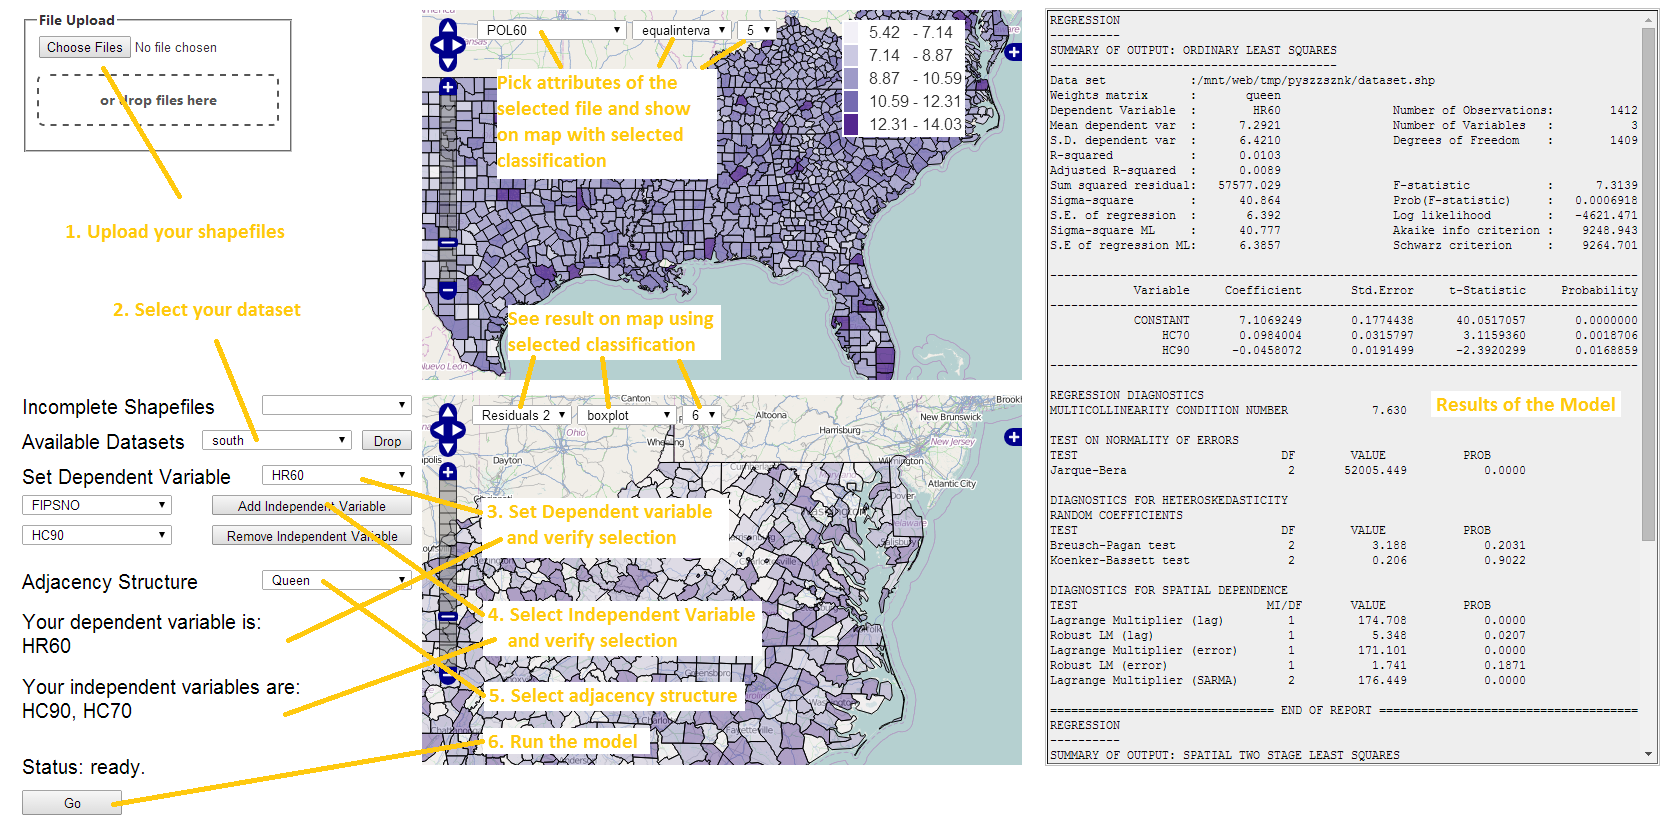
\includegraphics[width=.97\textwidth]{autoreg.png}\end{figure}
\end{frame}
}



{
\begin{frame}\frametitle{Model Path}

\begin{figure}
	\includegraphics[height=.97\textheight]{tree.png}\end{figure}
\end{frame}
}


\section*{Conclusion}

\begin{frame}\frametitle{Next Steps}
\begin{block}{Parallel Autoreg}
\begin{itemize}
	\item Ensemble of search strategies
	\begin{itemize}
		\item short
		\item full
		\item hybrid
	\end{itemize}
	\item Candidate Variables
	\item Candidate $W$s
\end{itemize}
\end{block}
\begin{block}{Integration}
\begin{itemize}
	\item CyberGIS Gateway
	\item Strategies
\end{itemize}
\end{block}
\alert{Come see the demo!}
\end{frame}
%\begin{frame}\frametitle{Next Steps}
%
%\begin{block}
%  \begin{itemize}
%	  \item Ensemble of search strategies
%	  \begin{itemize}
%		  \item Short
%		  \item Full
%	  \end{itemize}
%	  \item Candidate variables
%	  \item Candidate $W$s
%  \end{itemize}
%\end{block}
%%\begin{block}
%%  \begin{itemize}
%%	  \item Integration in Gateway
%%  \end{itemize}
%%\end{block}
%%\end{itemize}
%
%	


\end{document}
